\chapter{Finite Element Mehod (FEM)}

\section{Introduction}
The \textbf{Finite Element Method (FEM)} is a numerical technique for solving boundary value problems in engineering and mathematical physics. It subdivides a large problem into smaller, simpler parts called \textit{finite elements}, and then systematically reassembles them into a global solution.

Can be used for different types of analysis.
\begin{itemize}
\item Solid mechanics:
\begin{itemize}
  \item Static analysis;
  \item Dynamic analysis;
  \item Buckling analysis;
  \item Modal analysis;
\end{itemize}
\item Fluid mechanics;
\item Heat transfer;
\item Electromagnetic;
\end{itemize}



\section{Key Concepts}
\begin{itemize}
    \item \textbf{Domain Discretization:} The problem domain is divided into finite elements (triangles, quadrilaterals, tetrahedra, etc.), which careates a \textit{mesh}. There are also different dimentions the element can be, i.e., 1D:\ Line, 2D:\ surface, 3D:\ solid;
    \item \textbf{Field variables:} the forces afect the solid object in static analysis, e.,g stresses, strains, displacement.
    \item \textbf{Displacement vector:} each node, i.e., a connection point to antoher element, has some defrees of freedom that represents axial, bending, shear and torsional in the case of a lines element. For a line element the displacement vector $\{u\}$ will be $\{u_1, v_1, \theta_1, u_2, v_2, \theta_1\} ^T$, see figure~\ref{fig:displacement-vector}. Displacement vector $\{u\} = \{ u_1, v_1, w_1, \theta_{x1}, \theta_{y1}, \theta_{z1}, u_2, v_2, w_2, \theta_{x2}, \theta_{y2}, \theta_{z2}\} ^T$
    \item \textbf{Shape Functions:} Interpolation functions (often denoted by $\phi_i$) that approximate the solution within each element.
    \item \textbf{Weak Formulation:} The problem is reformulated into a \textit{weak} or \textit{variational form}, typically by applying the method of weighted residuals.
    \item \textbf{Stiffness Matrix:} A system of algebraic equations is derived from the weak form, resulting in a global stiffness matrix $\mathbf{K}$.
\end{itemize}

\begin{figure}[H]
  \centering
  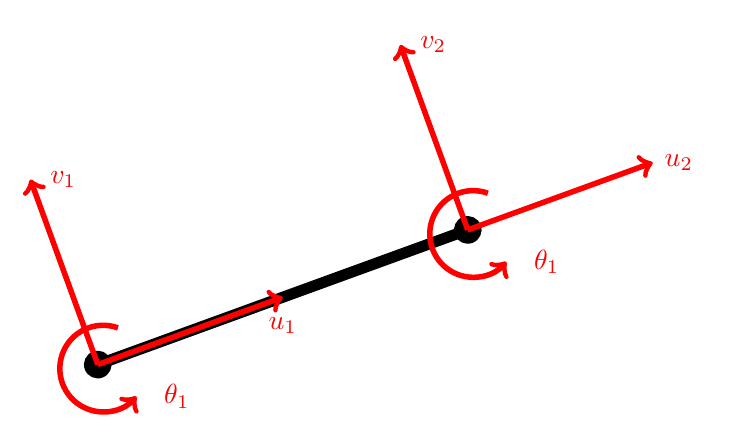
\begin{tikzpicture}

  \begin{scope}[rotate=20]
    \coordinate (p1) at (0,0);
    \coordinate (p2) at (5,0);

    \draw[line width=4pt] (p1) -- (p2);
    \fill (p1) circle (5pt);
    \fill (p2) circle (5pt);

    \draw[line width=2pt, red, ->] (p1) -- (2.5,0) node[below=1mm] {$u_1$};
    \draw[line width=2pt, red, ->] (p1) -- (0,2.5) node[right=1mm] {$v_1$};
    \draw[line width=2pt, red, ->] (p2) -- (7.5,0) node[right] {$u_2$};
    \draw[line width=2pt, red, ->] (p2) -- (5,2.5) node[right=1mm] {$v_2$};

    \draw[line width=2pt, red, ->] (0.4,0.35) arc[start angle=50, end angle=300, radius=5.5mm] node[right=2mm] {$\theta_1$};
    \draw[line width=2pt, red, ->] (5.4,0.35) arc[start angle=50, end angle=300, radius=5.5mm] node[right=2mm] {$\theta_1$};

  \end{scope}
  
  \end{tikzpicture}
  \caption{fig:displacement-vector}
\end{figure}

\section{Steps in FEM}
\begin{enumerate}
    \item \textbf{Discretization of the Domain:} Divide the domain into finite elements.
    \item \textbf{Selection of Shape Functions:} Choose shape functions $\phi_i$ to approximate the solution.
    \item \textbf{Derivation of Element Equations:} Formulate the element stiffness matrix $\mathbf{K}_e$ and force vector $\mathbf{F}_e$.
    \item \textbf{Assembly of Global System:} Assemble all element equations into a global system:
    \[
    \mathbf{K} \mathbf{u} = \mathbf{F}
    \]
    where $\mathbf{K}$ is the global stiffness matrix, $\mathbf{u}$ is the nodal displacement vector, and $\mathbf{F}$ is the global force vector.
    \item \textbf{Application of Boundary Conditions:} Apply constraints and boundary conditions to the system.
    \item \textbf{Solution of Algebraic Equations:} Solve the resulting system of equations for nodal values.
    \item \textbf{Post-Processing:} Compute derived quantities (stresses, strains) and visualize results.
\end{enumerate}

\section{Mathematical Formulation}
\textbf{Weak Form:} For a general PDE of the form:
$\mathcal{L}(u) = f \quad \text{in } \Omega$
with boundary conditions:
$u = u_D \quad \text{on } \Gamma_D \quad \text{and} \quad \nabla u \cdot \mathbf{n} = q \quad \text{on } \Gamma_N$
The weak form is:
$\int_{\Omega} \phi \mathcal{L}(u) \, d\Omega = \int_{\Omega} \phi f \, d\Omega + \int_{\Gamma_N} \phi q \, d\Gamma$
for all test functions $\phi$.

\section{Advantages and Applications}
\begin{itemize}
    \item \textbf{Advantages:}
    \begin{itemize}
        \item Can handle complex geometries and boundary conditions.
        \item Applicable to various types of problems (structural, thermal, fluid dynamics).
    \end{itemize}
    \item \textbf{Applications:}
    \begin{itemize}
        \item Structural analysis (stress and deformation).
        \item Heat transfer.
        \item Fluid flow.
        \item Electromagnetic fields.
    \end{itemize}
\end{itemize}

%%% Local Variables:
%%% TeX-master: "../../main"
%%% End:
